\documentclass[english,reprint, aps, prl,superscriptaddress, showpacs,
showkeys, longbibliography, amsmath, amssymb, floatfix]{revtex4-1} 
\pdfoutput=1

\usepackage{fullpage}
\usepackage{cmap}
\usepackage[T1,T2A]{fontenc}
\usepackage[utf8]{inputenc}
\usepackage[french,main=english]{babel}
\usepackage{amsthm}
\usepackage{mathrsfs}
\usepackage{bbold}
\usepackage{wesa}
\usepackage{graphicx}
\usepackage{verbatim}
\usepackage[backref=false]{hyperref}
\usepackage{booktabs}
\usepackage{multirow}
\usepackage[braket,qm]{qcircuit}
\usepackage{color}
\usepackage[usenames,dvipsnames]{xcolor}
\usepackage{framed}
\usepackage{comment}
\usepackage{xparse}

\theoremstyle{plain}
\newtheorem{thm}{Theorem}
\newtheorem{lemma}{Lemma}[thm]
\newtheorem{cor}{Corollary}[thm]
\newtheorem{assumption}{Assumption}
\newtheorem{fact}{Fact}
\theoremstyle{definition}
\newtheorem{definition}{Definition}
\newtheorem{condition}[assumption]{Condition}

\DeclareUnicodeCharacter{0229}{\c{e}}

\newcommand{\Hilb}{\mathcal{H}}
\newcommand{\events}{\ensuremath{\mathcal{E}}}
\newcommand{\qevents}{\ensuremath{\mathcal{E}}}
\newcommand{\pmeas}{\ensuremath{\mu}}
\newcommand{\imposs}{{\text{\wesa{impossible}}}}
\newcommand{\likely}{{\text{\wesa{likely}}}}
\newcommand{\unlikely}{{\text{\wesa{unlikely}}}}
\newcommand{\necess}{{\text{\wesa{certain}}}}
\newcommand{\unknown}{{\text{\wesa{unknown}}}}
\newcommand{\midd}{{\text{\wesa{middle}}}}
\newcommand{\fket}[1]{{|#1\rangle}}
\newcommand{\fproj}[1]{|#1\rangle\langle #1|}
\newcommand{\proj}[1]{\op{#1}{#1}}
\newcommand{\ps}{\texttt{+}}
\newcommand{\ms}{\texttt{-}}
\newcommand{\set}[2]{\ensuremath{\left\{ {#1}\mathrel{}\middle|\mathrel{}{#2}\right\} }}
\newcommand{\Tr}{\ensuremath{\mathop{\mathrm{Tr}}\nolimits}}
\allowdisplaybreaks
\newcommand{\coreBorn}{\ensuremath{\overline{\Hilb}}}
\newcommand{\mul}[1][]{\ensuremath{\mu^{L{#1}}}}
\newcommand{\mur}[1][]{\ensuremath{\mu^{R{#1}}}}
\setcounter{secnumdepth}{3}
% https://tex.stackexchange.com/questions/345284/can-i-have-an-almost-non-breaking-space-in-latex
% Change non-breaking space to \nolinebreak[1] 
% Hence, it will not hyphenate too much surrounding words.
\newcommand{\rmd}{d}
\newcommand{\rmi}{i}
\lineskiplimit=1pt
\newcommand{\ultramodular}{\mathcal{M}}
\newcommand{\ultramodularL}[1][]{\ensuremath{\ultramodular^{L{#1}}}}
\newcommand{\ultramodularR}[1][]{\ensuremath{\ultramodular^{R{#1}}}}
\newcommand{\muB}{\ensuremath{\mu^{B}}}
\newcommand{\eventsC}{\ensuremath{\events_{C}}}

\newcommand{\says}[3]{\begin{framed}\begin{minipage}{0.9\linewidth}\color{#1}{#2 says: #3}\end{minipage}\end{framed}}
\newcommand{\amr}[1]{\says{green}{Amr}{#1}}
\newcommand{\yutsung}[1]{\says{purple}{Yu-Tsung}{#1}}
\newcommand{\gerardo}[1]{\says{OliveGreen}{Gerardo}{#1}}
\newcommand{\andy}[1]{\says{blue}{Andy}{#1}}
% \excludecomment{suggest}
\NewDocumentEnvironment{suggest}{m m O{}}{#1{TEXT \##2 would go here. #3}}{#1{TEXT \##2 end here.}}

%%%%%%%%%%%%%%%%%%%%%%%%%%%%%%%%%%%%%%%%%%%%%%%%%%%%%%%%%%%%%%%%%%%
\begin{document}

\title{Response of the Referee Report of ``Quantum Interval-Valued Probability:
Contextuality and the Born Rule''}

\author{Yu-Tsung Tai}
\affiliation{Department of Mathematics, Indiana University, Bloomington, Indiana 47405,
USA}
\affiliation{Department of Computer Science, Indiana University, Bloomington,
Indiana 47405, USA}

\author{Andrew J. Hanson}
\affiliation{Department of Informatics, Indiana University, Bloomington,
Indiana 47405, USA}

\author{Gerardo Ortiz}
\affiliation{Department of Physics, Indiana University, Bloomington, Indiana 47405,
USA}

\author{Amr Sabry}
\affiliation{Department of Computer Science, Indiana University, Bloomington,
Indiana 47405, USA}

\date{\today}

\maketitle

%%%%%%%%%%%%%%%%%%%%%%%%%%%%%%%%%%%%%%%%%%%%%%%%%%%%%%%%%%%%%%%%%%%
\subsection{Classical $\frac{1}{4}$-deterministic Probability Measure}

Although the definition of $\delta$-determinism in our paper only
applied on QIVPMs~\cite{THOS2017}, this definition can be easily
extended to apply on both classical and quantum IVPMs as follow.

\begin{definition}[$\delta$-Determinism]\label{def:delta-deterministic}
Given a classical or quantum IVPM~$\bar{\mu}:\events'\rightarrow\mathscr{I}$,
where $\events'$ is the set of all events, $\events$, when $\bar{\mu}$
is a QIVPM and $\events'$ is the set of mutually commuting events,
$\eventsC$, when $\bar{\mu}$ is a classical one. Then, $\bar{\mu}$
is $\delta$-deterministic if, for every event $P\in\events'$, we
have that either $\bar{\mu}\left(P\right)\subseteq\left[0,\delta\right]$
or $\bar{\mu}\left(P\right)\subseteq\left[1-\delta,1\right]$. \end{definition}

\begin{table}
\noindent \centering{}\caption{\label{tab:classical-IVPMs}Examples of $\delta$-deterministic classical
IVPMs $\bar{\mu}_{A}$ and $\bar{\mu}_{B}$ on commuting events $P$.}
\begin{tabular}{ccc}
\toprule 
\addlinespace
$P$  & $\bar{\mu}_{A}(P)$  & $\bar{\mu}_{B}(P)$ \tabularnewline
\midrule
\midrule 
\addlinespace
$\mathbb{0}$  & $\imposs$  & $\imposs$ \tabularnewline
\midrule 
\addlinespace
$\proj{0}$  & $\necess$  & $\left[\frac{3}{4},\frac{4}{5}\right]$ \tabularnewline
\midrule 
\addlinespace
$\proj{1}$  & $\imposs$  & $\left[\frac{1}{5},\frac{1}{4}\right]$ \tabularnewline
\midrule 
\addlinespace
$\mathbb{1}$  & $\necess$  & $\necess$ \tabularnewline
\bottomrule
\end{tabular}
\end{table}

\noindent Then, it is easy to construct $\delta$-deterministic classical
IVPMs $\bar{\mu}_{A}$ and $\bar{\mu}_{B}$ defined in Table~\ref{tab:classical-IVPMs},
where $\proj{0}$ and $\proj{1}$ represents heads and tails in coin-tossing,
respectively. The interpretation for $\bar{\mu}_{A}$ is that we have
a double-headed coin that always lands on head. For $\bar{\mu}_{B}$,
the interpretation is that we throw a coin $1000$ times and we observe
$750$ heads and $200$ tails and the coin falls under the couch $50$
times. For $\bar{\mu}_{A}$, $\delta$ is $0$; for $\bar{\mu}_{B}$,
$\delta=\frac{1}{4}$, and $\delta$ qualifies how a coin close to
double-headed, which we can certainly know the outcome of an coin
even before tossing. We see here that we can construct $0$-deterministic
as well as $\frac{1}{4}$-deterministic and in fact for any $\delta$
in the range $\left[0,1\right]$ we can construct a $\delta$-deterministic
classical probability measure. BUT the situation changes in the quantum
case, WE CANNOT construct $\delta$-deterministic probability measures
for $\delta<\frac{1}{3}$.

\subsection{Why a Quantum $\frac{1}{4}$-deterministic Probability Measure is
Impossible}

To illustrate our proof for non-existence of $\delta$-deterministic
QIVPMs for $\delta<\frac{1}{3}$, we will explain why we cannot construct
any $\frac{1}{4}$-deterministic QIVPM in full details. The proof
is by contradiction: Suppose there is a $\frac{1}{4}$-deterministic
QIVPM~$\bar{\mu}:\events\rightarrow\mathscr{I}$. Now use this assumed
QIVPM to construct the following $0$-deterministic QIVPM $\bar{\mu}^{\textrm{D}}:\events\rightarrow\left\{ \imposs,\necess\right\} $:
\begin{equation}
\bar{\mu}^{\textrm{D}}\left(P\right)=\begin{cases}
\imposs\,, & \textrm{ if }\bar{\mu}\left(P\right)\subseteq\left[0,\tfrac{1}{4}\right]\:;\\
\necess\,, & \textrm{ if }\bar{\mu}\left(P\right)\subseteq\left[\tfrac{3}{4},1\right]\:.
\end{cases}
\end{equation}
However, since we know that $0$-deterministic QIVPMs do not exist,
the map $\bar{\mu}^{\textrm{D}}$ cannot exist and hence $\bar{\mu}$
does not exist. It remains to verify that $\bar{\mu}^{\textrm{D}}$
is indeed a QIVPM. Since the range of $\bar{\mu}^{\textrm{D}}$, $\left\{ \imposs,\necess\right\} $,
is a set of singleton sets, if $\bar{\mu}^{\textrm{D}}$ satisfies
that for orthogonal projectors~$P_{0}$ and $P_{1}$, 
\begin{equation}
\bar{\mu}^{\textrm{D}}\left(P_{0}+P_{1}\right)=\bar{\mu}^{\textrm{D}}\left(P_{0}\right)+\bar{\mu}^{\textrm{D}}\left(P_{1}\right)\,,\label{eq:QuantumInterval-valuedProbability-Equal}
\end{equation}
then we can apply the same reason of proving classical inclusion-exclusion
principle~\cite{TaiThesis2018} to get
\[
\bar{\mu}^{\textrm{D}}\left(P_{0}+P_{1}-P_{0}P_{1}\right)+\bar{\mu}^{\textrm{D}}\left(P_{0}P_{1}\right)=\bar{\mu}^{\textrm{D}}\left(P_{0}\right)+\bar{\mu}^{\textrm{D}}\left(P_{1}\right)
\]
which implies $\bar{\mu}^{\textrm{D}}$ is convex, i.e., $\bar{\mu}^{\textrm{D}}$
is a QIVPM. Therefore, our task now is to prove Eq.~(\ref{eq:QuantumInterval-valuedProbability-Equal}).

\begin{figure*}
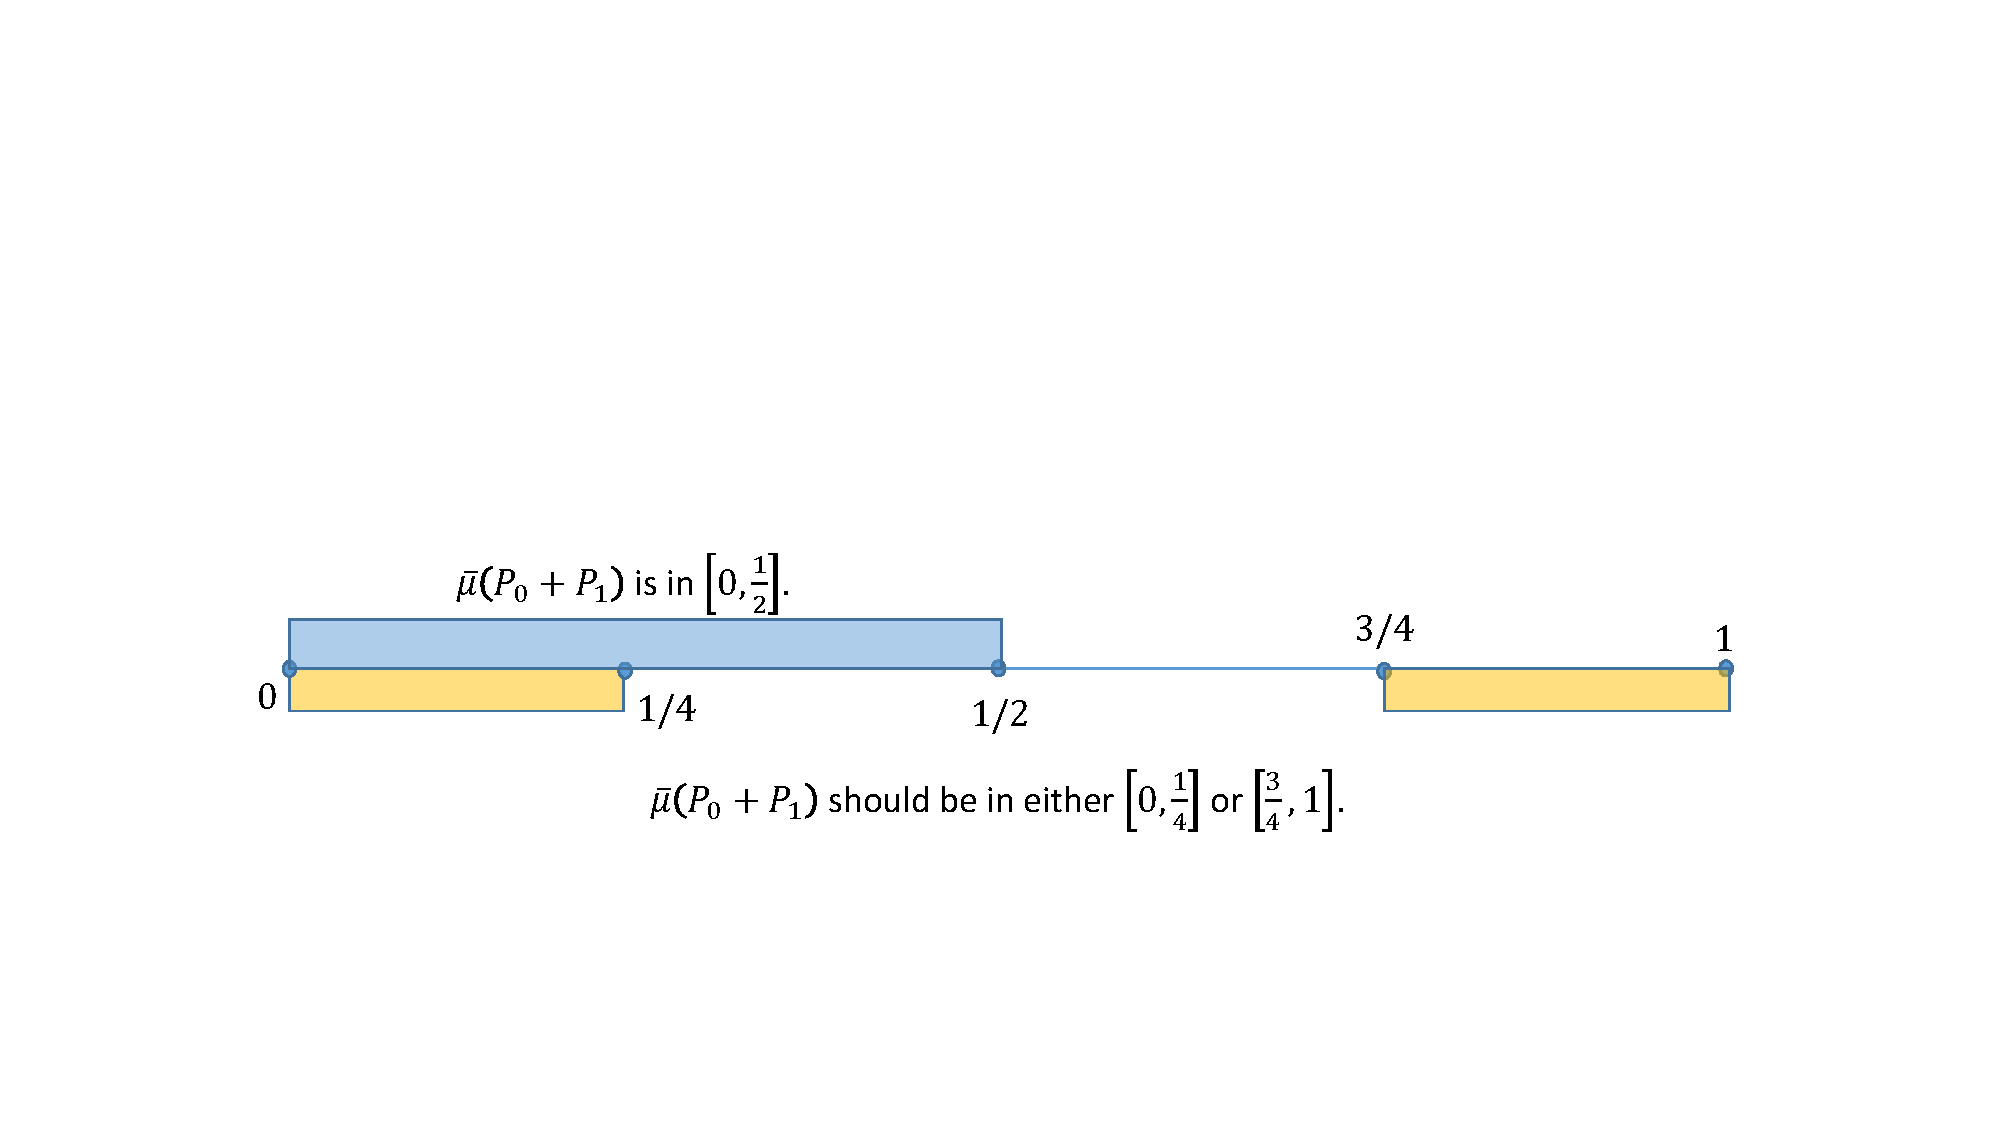
\includegraphics[bb=50bp 100bp 900bp 300bp,clip,scale=0.5]{prop_prop_letter_ajhs_referee_response_pptx}\caption{\label{fig:Show-subset}Show $\bar{\mu}\left(P_{0}+P_{1}\right)$
must be a subset of $\left[0,\frac{1}{4}\right]$.}
\end{figure*}
For orthogonal projectors~$P_{0}$ and $P_{1}$, when one of $\bar{\mu}^{\textrm{D}}\left(P_{0}\right)$
and $\bar{\mu}^{\textrm{D}}\left(P_{1}\right)$ is $\necess$, say
$\bar{\mu}^{\textrm{D}}\left(P_{0}\right)=\necess$. Then, $\bar{\mu}^{\textrm{D}}\left(P_{1}\right)=\imposs$,
$\bar{\mu}\left(P_{0}\right)\subseteq\left[\frac{3}{4},1\right]$,
$\bar{\mu}\left(P_{1}\right)\subseteq\left[0,\frac{1}{4}\right]$,
and $\bar{\mu}\left(P_{0}+P_{1}\right)\subseteq\left[\frac{3}{4},\frac{5}{4}\right]$.
Since $\bar{\mu}\left(P_{0}+P_{1}\right)$ is bounded by $\left[0,1\right]$,
we must have $\bar{\mu}\left(P_{0}+P_{1}\right)\subseteq\left[\frac{3}{4},1\right]$,
i.e., $\bar{\mu}^{\textrm{D}}\left(P_{0}+P_{1}\right)=\necess=\bar{\mu}^{\textrm{D}}\left(P_{0}\right)+\bar{\mu}^{\textrm{D}}\left(P_{1}\right)$.

For orthogonal projectors~$P_{0}$ and $P_{1}$, when $\bar{\mu}^{\textrm{D}}\left(P_{0}\right)=\bar{\mu}^{\textrm{D}}\left(P_{1}\right)=\imposs$,
we have both $\bar{\mu}\left(P_{0}\right)$ and $\bar{\mu}\left(P_{1}\right)\subseteq\left[0,\frac{1}{4}\right]$
which implies $\bar{\mu}\left(P_{0}+P_{1}\right)\subseteq\left[0,\frac{1}{2}\right]$.
Since $\bar{\mu}\left(P_{0}+P_{1}\right)$ is a subset of either $\left[0,\frac{1}{4}\right]$
or $\left[\tfrac{3}{4},1\right]$ and the latter is excluded as illustrated
in Fig.~\ref{fig:Show-subset} , then $\bar{\mu}\left(P_{0}+P_{1}\right)$
must be a subset of $\left[0,\frac{1}{4}\right]$, which implies $\bar{\mu}^{\textrm{D}}\left(P_{0}+P_{1}\right)=\imposs$.

%%%%%%%%%%%%%%%%%%%%%%%%%%%%%%%%%%%%%%%%%%%%%%%%%%%%%%%%%%%%%%%%%%%%%%%%%%%%%
\bibliography{prop}
\end{document}

